%-----------------------------------
%   PROTOCOLO DE AUTOCONFIGURACIÓN DE DIRECCIONES PROPUESTO
%-----------------------------------
\chapter{Protocolo de autoconfiguración de direcciones propuesto}

\label{ch:autoconfiguracion_de_direcciones_propuesto}

Como se mencionó en el capítulo \ref{ch:autoconfiguracion_de_direcciones}, para
que los vehículos puedan comunicarse a través de la red, necesitan tener una
dirección IP. Al no contar con un servidor DHCP que se encargue de asignar una
dirección a cada vehículo, se requiere de un método que le permita a cada
vehículo obtener una dirección IP única de manera autónoma.

La razón por la que las direcciones IP tienen una estructura jerárquica, es que,
de este modo, los dispositivos que forman una red grande se pueden agrupar para
formar subredes, y esto facilita el enrutamiento. En las redes cableadas, la
jerarquización está determinada por la topología de la red. No obstante, en una
VANET, la topología cambia constantemente, por lo que se debe utilizar otro
método para agrupar a los vehículos y formar las subredes. En el presente
capítulo, se describe el protocolo de autoconfiguración de direcciones que se
diseñó para lograr este objetivo.

%-----------------------------------
%   FORMACIÓN DE LAS SUBREDES
%-----------------------------------
\section{Formación de las subredes}

\label{sec:formacion_de_subredes}

Una dirección IP se forma por dos partes, como se explica en la sección
\ref{subsec:direccionamiento_ipv6}: el prefijo, que identifica a la subred, y el
identificador asignado a la interfaz. Para que un vehículo pueda obtener una
dirección, lo primero que necesita conocer es la subred a la que se va a unir.
Esto nos lleva al problema de cómo agrupar a los vehículos para formar las
subredes.

Debido a las restricciones del canal de comunicación inalámbrica, como el
radio de transmisión, los vehículos se agrupan geográficamente. Es decir, una
subred se debe formar por el subconjunto de vehículos que se encuentran dentro
de cierta región geográfica. Si un vehículo es capaz de conocer su ubicación,
puede determinar en qué región se encuentra, y, por lo tanto, cuál es la red a
la que debe unirse. Por este motivo, se requiere que todos los vehículos
cuenten con algún dispositivo que les permita obtener su ubicación geográfica.

Después de definir la manera en la que se van a agrupar los vehículos para
formar las subredes, se debe especificar cómo se determinarán los límites de
cada región, y cómo asignar un código con el que se pueda generar el prefijo de
la subred para cada una. Para lograr esto, se recurrió al sistema de
codificación Geohash, que se describe en la siguiente sección.

%-----------------------------------
%   CODIFICACIÓN GEOHASH
%-----------------------------------
\subsection{Codificación Geohash}

\label{subsec:codificacion_geohash}

En el sistema de codificación Geohash, se representa una ubicación o una
región geográfica con una cadena corta de letras y números. La longitud del
codigo determina la precisión de la ubicación. Además, esta codificación permite
saber si dos ubicaciones son cercanas analizando la longitud del prefijo común
entre sus códigos \cite{wiki:Geohash}.

Un código Geohash es una cadena binaria, que se convierte en una secuencia de
símbolos de la codificación base 32, que se muestra en la tabla
\ref{tab:base32}.

\begin{table}[th]
\centering
\caption{Codificación base 32.}
\label{tab:base32}
\begin{tabular}{c c}
\toprule
\tabhead{Binario} & \tabhead{Base 32} \\
\midrule
00000 & 0 \\
00001 & 1 \\
00010 & 2 \\
00011 & 3 \\
00100 & 4 \\
00101 & 5 \\
00110 & 6 \\
00111 & 7 \\
01000 & 8 \\
01001 & 9 \\
01010 & b \\
01011 & c \\
01100 & d \\
01101 & e \\
01110 & f \\
01111 & g \\
\bottomrule
\end{tabular}
\quad
\begin{tabular}{c c}
\toprule
\tabhead{Binario} & \tabhead{Base 32} \\
\midrule
10000 & h \\
10001 & j \\
10010 & k \\
10011 & m \\
10100 & n \\
10101 & p \\
10110 & q \\
10111 & r \\
11000 & s \\
11001 & t \\
11010 & u \\
11011 & v \\
11100 & w \\
11101 & x \\
11110 & y \\
11111 & z \\
\bottomrule
\end{tabular}
\end{table}

Para formar un código Geohash, se divide toda la superficie de la Tierra en 32
celdas (figura \ref{fig:geohash1}), y a cada una se le asigna un símbolo. Se
elige la región que contiene la ubicación de interés y se agrega el símbolo
correspondiente al código. La región seleccionada se divide en 32 celdas (figura
\ref{fig:geohash2}), y nuevamente se selecciona la que contiene la ubicación, y
su símbolo se agrega al código. Este proceso se repite hasta obtener la
precisión necesaria. Se puede notar que, mientras más largo sea el prefijo
común entre dos códigos, más cercanas entre sí son las ubicaciones que
representan. En el apédice \ref{app:b} se explica con más detalle cómo
codificar una ubicación para obtener un código Geohash.

\begin{figure}[th!]
\centering
\includegraphics[width=0.85\textwidth]{geohash1} 
\decoRule
\caption[Códio Geohash de longitud 1]{Códio Geohash de longitud 1.}
\label{fig:geohash1}
\end{figure}

\begin{figure}[th!]
\centering
\includegraphics[width=0.85\textwidth]{geohash2}
\decoRule
\caption[Códio Geohash de longitud 2]{Códio Geohash de longitud 2.}
\label{fig:geohash2}
\end{figure}

Un mismo código se puede interpretar con una región o como una ubicación, en
cuyo caso, generalmente, se considera el centro de la región. En la tabla
\ref{tab:tamaño_celdas_geohash} se muestra el tamaño aproximado de las celdas
que se obtienen de acuerdo a la longitud del código. Se debe considerar que el
tamaño de las celdas es más pequeño a medida de que se alejan del ecuador
\cite{GeohashBolivia}.

\begin{table}[th]
\caption{Tamaño de las celdas para diferentes longitudes de código
\cite{GeohashBolivia}.}
\label{tab:tamaño_celdas_geohash}
\centering
\begin{tabular}{c c r r}
\toprule
\tabhead{Longitud del código} & & \tabhead{Ancho} & \tabhead{Alto}\\
\midrule
1 & $\leq$ & 5,000 km & 5,000 km\\
2 & $\leq$ & 1,250 km & 625 km\\
3 & $\leq$ & 156 km & 156 km\\
4 & $\leq$ & 39.1 km & 19.5 km\\
5 & $\leq$ & 4.89 km & 4.89 km\\
6 & $\leq$ & 1.22 km & 0.61 km\\
7 & $\leq$ & 153 m & 153 m\\
8 & $\leq$ & 38.2 m & 19.1 m\\
9 & $\leq$ & 4.77 m & 4.77 m\\
10 & $\leq$ & 1.19 m & 0.596 m\\
11 & $\leq$ & 149 mm & 149 mm\\
12 & $\leq$ & 37.2 mm & 18.6 mm\\
\bottomrule\\
\end{tabular}
\end{table}

A partir de aquí, se llamará código \textbf{Geohash-\textit{n}} a un código
Geohash de longitud \textit{n}. También, se entenderá como \textbf{región
Geohash} o \textbf{ubicación Geohash} a una región o ubicación, respectivamente,
representadas por un código Geohash.

% La división de las regiones se hace con base en la división que se deriva de
% este sistema de codificación. La longitud de códigos que se usa es 6, por lo que
% las regiones resultantes miden aproximadamente 1.22 km en longitud y 0.61
% km en latitud, según la tabla \ref{tab:tamaño_celdas_geohash}. Este tipo de
% códigos se pueden traducir de manera directa a cadenas de bits, por lo que se
% peden incorporar fácilmente a las direcciones IP. Cada símbolo del código se
% convierte en una secuencia de 5 bits, así que la longitud total del código es de
% 30 bits. Cuando un vehículo necesita saber en qué región se encuentra, calcula
% el código Geohash de su ubicación con una precisión de 6 símbolos, con lo que
% genera el identificador de subred para su dirección \textit{unicast} y el
% identificador de grupo para la dirección \textit{multicast}.

%-----------------------------------
%   SUBREDES GEOHASH
%-----------------------------------
\subsection{Subredes Geohash}

\label{subsec:subredes_geohash}

La codificación Geohash nos permite delimitar regiones y asociar un código a
cada una, por lo que sirve para resolver el problema planteado al final de la
sección \ref{sec:formacion_de_subredes}. Por esta razón, denominamos como
\textbf{subred Geohash} a una subred formada por los vehículos que se encuentran
dentro de una región Geohash. Ahora, se debe definir de qué tamaño deben ser
estas regiones.

Si las regiones fueran muy grandes, habría muy pocas subredes con muchos
vehículos cada una, por lo que no se aprovecharía la jerarquización de
direcciones que ofrece el protocolo IPv6, y esto complicaría el enrutamiento.
En la figura \ref{fig:region_geohash5} se puede notar que las regiones
Geohash-5 abarcan un área muy grande, por lo que se presentaría esta situación
si se eligiera este tamaño.

Por otra parte, si las regiones fueran muy pequeñas, habría muchas subredes con
muy pocos vehículos. En la figura \ref{fig:region_geohash7} podemos ver que las
regiones Geohash-7 son tan pequeñas, que algunas apenas abarcan un pequeño
segmento de alguna calle. Si se eligiera este tamaño, en algunos casos
podría llegar a haber regiones sin ningún vehículo. Además, algunos pares de
celdas adyacentes no cuentan con algún segmento de calle que las conecte, por
lo que los vehículos no podrían pasar de una región a otra.

Según la tabla \ref{tab:tamaño_celdas_geohash}, las regiones Geohash-6 son de
1.22 km de ancho y 0.61 km de alto, aproximadamente. En la figura
\ref{fig:region_geohash6} se puede ver que estas regiones tienen un tamaño más
apropiado que los de las regiones consideradas anteriormente.
Además, todas las regiones tienen al menos un segmento de calle que
las conecte con las cuatro regiones adyacentes. Es por esto que se decidió que
cada subred Geohash abarcará una región Geohash-6.

\begin{figure}[th!]
\centering

\begin{subfigure}{\textwidth}
\centering
\includegraphics[height=4cm]{region_geohash5} 
\caption[Regiones Geohash-5]{Regiones Geohash-5.}
\label{fig:region_geohash5}
\end{subfigure}

\vspace{0.5cm}

\begin{subfigure}{\textwidth}
\centering
\includegraphics[height=4cm]{region_geohash6} 
\caption[Regiones Geohash-6]{Regiones Geohash-6.}
\label{fig:region_geohash6}
\end{subfigure}

\vspace{0.5cm}

\begin{subfigure}{\textwidth}
\centering
\includegraphics[height=4cm]{region_geohash7} 
\caption[Regiones Geohash-7]{Regiones Geohash-7.}
\label{fig:region_geohash7}
\end{subfigure}

\vspace{0.5cm}

\decoRule
\caption[Tamaños de regiones Geohash]{Tamaños de regiones Geohash.}
\label{fig:tamaños_geohash}

\end{figure}

Ya que se tiene definido el tamaño de cada región, en las siguientes
secciones se describe cómo se utilizan los códigos Geohash de cada una para
determinar formar las direcciones IP con las que los vehículos podrán
autoconfigurarse.

%-----------------------------------
%   FORMATO DE LAS DIRECCIONES IPV6 UNICAST
%-----------------------------------
\subsection{Formato de las direcciones IPv6 \textit{unicast}}

\label{subsec:formato_direcciones_ipv6_unicast}

Para que un vehículo pueda compartir paquetes con otro, ambos necesitan tener
una dirección IP \textit{unicast}. Este tipo de direcciones identifican de
manera única a un dispositivo dentro de una red. El protocolo IPv6 define
diferentes tipos de direcciones \textit{unicast}, que se describen a
continuación \cite{CiscoIpv62011}:

\keyword{Dirección global agregable} -- Estas direcciones tienen un prefijo de
enrutamiento global de 48 bits que comienza con \code{2000::/3}. En seguida,
tiene un identifiador de subred de  16 bits, y al final el identificador del
nodo de 64 bits. Su asignación depende de la Autoridad de Asignación de Números
de Internet (IANA) y los proveedores de servicio de Internet (ISPs).

\keyword{Dirección local de enlace} --  Se pueden configurar automáticamente con
el prefijo \code{FE80::/10} y el identificador de la interfaz con el formato
EUI-64 (\ref{app:a}). Se usa para el protocolo de descubrimiento de vecinos y
el proceso de autoconfiguración sin estado. Los paquetes destinados a este tipo de
dirección no son enrutados.

\keyword{Dirección compatible con IPv4} -- Son direcciones que comienzan con el
prefijo \code{::/96} seguido de una dirección IPv4 de 32 bits. Se asignan a
nodos que sportan tanto IPv4 como IPv6.

\keyword{Dirección local única} -- Inician con el prefijo \code{FC00::/7}. Son
direcciones únicas globalmente, y son destinadas únicamente para comunicación
local; es decir, no se enrutan hacia Internet. Su asignación no depende del ISP
o de alguna otra entidad reguladora.

Debido a que no hay restricciones para la asignación de direcciones locales
únicas, este es el tipo de dirección \textit{unicast} que se usarán para
identificar a los vehículos. La figura \ref{fig:formato_direccion_unicast}
muestra el formato de una dirección local única \cite{CiscoIpv62011}.

\begin{figure}[th!]
\centering
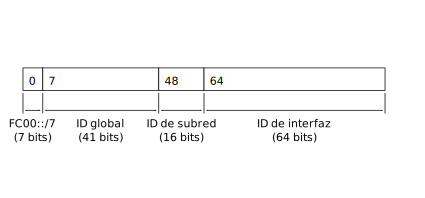
\includegraphics{formato_direccion_unicast}
\decoRule
\caption[Formato de una dirección local única]{Formato de una dirección
local única.}
\label{fig:formato_direccion_unicast}
\end{figure}

El identificador de la subred contiene el código Geohash asociado a esta, por
lo que las direcciones \textit{unicast} se denominan \keyword{direcciones
\textit{unicast} Geohash}. El formato destas direcciones se muestra en la
figura \ref{fig:formato_direccion_unicast_geohash}, y se conforma de la
siguiente manera:

\begin{figure}[th!]
\centering
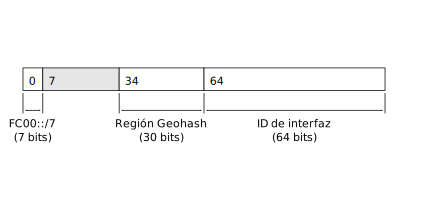
\includegraphics{formato_direccion_unicast_geohash}
\decoRule
\caption[Formato de una dirección \textit{unicast} Geohash]{Formato de una
dirección \textit{unicast} Geohash.}
\label{fig:formato_direccion_unicast_geohash}
\end{figure}

\keyword{Bits 0 - 6} -- Prefijo \code{FC00::/7}, que indica que se trata de
una dirección local única.

\keyword{Bits 7 - 33} -- No se usan; se fijan en 0.

\keyword{Bits 34 - 63} -- Código Geohash de la subred. Cuando un vehículo
conoce su ubicación, calcula el código Geohash, y los primeros 6 símbolos
corresponden al código de la subred. Este código se convierte a una cadena de
30 bits, de acuerdo con la tabla \ref{tab:base32}.

\keyword{Bits 64 - 127} -- Identificador de la interfaz en el formato
EUI-64.

%-----------------------------------
%   FORMATO DE DIRECCIONES IPV6 MULTICAST
%-----------------------------------
\subsection{Formato de direcciones IPv6 \textit{multicast}}

\label{subsec:formato_direcciones_ipv6_multicast}

Además de una dirección \textit{unicast}, cada vehículo necesita unirse a un
grupo \textit{multicast} para poder comunicarse con los demás de su misma
subred. En el protocolo IPv6, una dirección \textit{multicast} se forma por dos
partes: el prefijo \code{FF02::/16}, como se muestra en la figura
\ref{fig:formato_direccion_multicast}.

\begin{figure}[th!]
\centering
\includegraphics{formato_direccion_multicast}
\decoRule
\caption[Formato de una dirección \textit{multicast}]{Formato de una dirección
\textit{multicast}.}
\label{fig:formato_direccion_multicast}
\end{figure}

La dirección \textit{multicast} de cada subred también incluye el código
Geohash de esta, por lo que las direcciones \textit{mutlicast} se denominan
\keyword{direcciones \textit{multicast} Geohash}. El formato de estas
direcciones se muestra en la figura
\ref{fig:formato_direccion_multicast_geohash}, y se conforma de la siguiente
manera:

\keyword{Bits 0 - 15} -- Prefijo \code{FF02::/16}, que indica que se trata
de una dirección multicast.

\keyword{Bits 16 - 97} -- No se usan; se fijan en 0.

\keyword{Bits 98 - 127} -- Código Geohash de la subred. Cuando un vehículo
conoce su ubicación, calcula el código Geohash, y los primeros 6 símbolos
corresponden al código de la subred. Este código se convierte a una cadena de
30 bits, de acuerdo con la tabla \ref{tab:base32}.

\begin{figure}[th!]
\centering
\includegraphics{formato_direccion_multicast_geohash}
\decoRule
\caption[Formato de la dirección \textit{multicast} para cada región]{Formato de
la dirección \textit{multicast} para cada región.}
\label{fig:formato_direccion_multicast_geohash}
\end{figure}

%-----------------------------------
%   CAMBIO DE SUBRED
%-----------------------------------
\section{Cambio de subred}

\label{sec:cambio_subred}

Cuando un vehículo enciende su interfaz de red, lo único que necesita para
autoconfigurarse es conocer su ubicación. Con este dato, podrá obtener su
dirección \textit{unicast} y su dirección \textit{multicast}, como se explicó
en la sección anterior. Sin embargo, se necesita definir cómo llevará a cabo la
autoconfiguración cuando se mueva de una región Geohash a otra.

Si un vehículo, al consultar su ubicación, detecta que se encuentra en una nueva
región Geohash, lo más simple sería eliminar de la configuración de su interfaz
las direcciones \textit{unicast} y \textit{multicast} de la subred anterior, y
configurar las direcciones para unirse a la nueva subred. Pero, de este modo,
las subredes estarían completamente aisladas una de otra, por lo que no se
podría hacer un enrutamiento a través de varias subredes.

En la figura \ref{fig:gateways}, se muestra la frontera entre las subredes
A y B. Durante el enrutamiento, un paquete necesita ser transmitido del vehículo
A$_1$ al vehículo B$_1$. Para esto, A$_1$ primero debe transmitirlo a A$_2$,
que se encuentra en su misma subred. Después, A$_2$ debe retransmitirlo a B$_2$,
a pesar de que pertenecen a redes distintas. Finalmente, B$_2$ lo retransmite
hacia B$_1$, que está en su misma subred. Los vehículos A$_2$ y B$_2$ se
denominan \textbf{\textit{gateways}}.

\begin{figure}[th]
\centering
\includegraphics[width=8cm]{gateways}
\decoRule
\caption[Transmisión de paquetes de una subred a otra]{Transmisión de paquetes
de una subred a otra.}
\label{fig:gateways}
\end{figure}

Cuando un vehículo se encuentra dentro de los límites de una región Geohash, y
forma parte de la subred correspondiente a esa región, esta se denomina como
\textbf{subred primaria} del vehículo. La región resaltada de color gris en la
figura \ref{fig:gateways} se denota \textbf{región \textit{gateway}}.
Cuando un vehículo entra a la región \textit{gateway}, se auto-asigna las
direcciones \textit{unicast} y \textit{multicast} correspondientes a la subred
vecina. En el momento en que el vehículo forma parte también de la subred
vecina, esta se llama \textbf{subred secundaria} del vehículo. En la figura
\ref{fig:gateways}, el nodo A$_1$ tiene como subred primaria la subred A, y
no tiene subred secundaria, ya que no se encuentra dentro de la región gateway.
Para el nodo A$_2$, la subred primaria es la subred A, y la subred secundaria es
la B. Para el nodo B$_2$, la subred primaria es la B, y la secundaria es la A; y
para el nodo B$_1$, la subred primaria es la B, y no tiene subred secundaria.

Un \textit{gateway} deben tener la capacidad de recibir y transmitir paquetes
desde y hacia una subred vecina, por lo que debe ser parte de dos subredes a la
vez. Cualquier vehículo puede ser un \textit{gateway} si se encuentra cerca de
la frontera entre dos subredes. En el momento en que un vehículo se encuentre a
cierta distancia de la frontera, éste informa a los demás vehículos que se ha
convertido en un \textit{gateway}. Así, los demás podrán saber que a través de
él pueden transmitir paquetes hacia la subred vecina.

A continuación, se describe el procedimiento que lleva a cabo un vehículo cuando
se mueve de una subred a otra.

\begin{enumerate}
  \item El vehículo se encuentra dentro de una región Geohash, y su subred
  primaria es la correspondiente a la región. En la figura
  \ref{fig:cambio_subred1}, la subred primaria es la A.
  \item El vehículo entra a la región \textit{gateway} de la región Geohash
  donde se encuentra. En este momento, se une a la subred vecina como subred
  secundaria, y sigue siendo parte de la subred primaria. En la figura
  \ref{fig:cambio_subred2}, la subred secundaria es la B.
  \item El vehículo sale de la primera región Geohash y entra a la región
  \textit{gateway} de la nueva región. Aquí, la subred secundaria pasa a ser la
  región primaria --ya que ahora se encuentra físicamente en la nueva región--,
  y la región primaria pasa a ser la región secundaria. Sin embargo, todavía
  forma parte de ambas subredes. En la figura \ref{fig:cambio_subred3}, ahora la
  subred primaria es la B y la subred secundaria es la A.
  \item El vehículo sale de la región \textit{gateway} de la nueva región. A
  partir de aquí, el vehículo deja de pertenecer a la subred secundaria, ya que
  no es \textit{gateway} hacia ninguna otra subred. En la figura
  \ref{fig:cambio_subred4}, la subred primaria del vehículo es la B, y ya no
  tiene subred secundaria.
\end{enumerate}

\begin{figure}[th]
\centering

\begin{subfigure}{\textwidth}
\centering
\includegraphics[width=8cm]{cambio_subred1} 
\caption[Vehículo dentro de la primera región Geohash.]{Vehículo dentro de la
primera región Geohash.}
\label{fig:cambio_subred1}
\end{subfigure}

\vspace{0.5cm}

\begin{subfigure}{\textwidth}
\centering
\includegraphics[width=8cm]{cambio_subred2} 
\caption[El vehículo entra a la región \textit{gateway}.]{El vehículo entra a la
región \textit{gateway}.}
\label{fig:cambio_subred2}
\end{subfigure}

\vspace{0.5cm}

\begin{subfigure}{\textwidth}
\centering
\includegraphics[width=8cm]{cambio_subred3} 
\caption[El vehículo se mueve de una región Geohash a otra.]{El vehículo se
mueve de una región Geohash a otra.}
\label{fig:cambio_subred3}
\end{subfigure}

\vspace{0.5cm}

\begin{subfigure}{\textwidth}
\centering
\includegraphics[width=8cm]{cambio_subred4} 
\caption[El vehículo sale de la región \textit{gateway}.]{El vehículo sale de
la región \textit{gateway}.}
\label{fig:cambio_subred4}
\end{subfigure}

\vspace{0.5cm}

\decoRule
\caption[Vehículo cambiando de una subred a otra]{Vehículo cambiando de una
subred a otra.}
\label{fig:cambio_subred}

\end{figure}

